% !TEX root = ../thesis_main.tex
\chapter{Effects of a reduced order model for protein representation}
\graphicspath{{rom_studies/figs/}}

Part of the process of computational modelling is making assumptions about the problem we are trying to solve. In the 
field of localized surface plasmon resonance for biosensing applications there are several research papers that use Bovine Serum Albumin 
as an analyte to simulate the behavior of a bioconjugate sensor. However, they use extremely simplified models
to represent the protein, and often a real-valued dielectric for the medium. Some models consist of  
a layer of protein-water solution \cite{PhanETal2013}, 
or just a protein dielectric layer \cite{NghiemETal2012}, others model the
protein as a triangular prism \cite{DanHu2014}, or even a small sphere with a 
constant dielectric \cite{AntosiewiczApellClaudioKall2011, DavisGomezVernon2010,SantiagoCordobaETal2011, UngerETal2009}. Phan and 
coworkers \cite{PhanETal2013} present a Lorentz-Drude model for the complex 
dielectric of the BSA which we use in our work, while most of the literature 
use a constant dielectric with no losses to represent the BSA 
(refractive index of $n= 1.9$ \cite{NghiemETal2012}, $n= 1.45$ \cite{SantiagoCordobaETal2011}) or
other proteins used as analytes ($n=1.58$ polystrene \cite{UngerETal2009}, $n=1.57$ 
streptavidin \cite{ShenETal2013}). 

Research shows that the shape of both monomer and dimmer of BSA are prolate ellipsoids 
\cite{MoserETal1966, SquireETal1968, WrightETal1975}. However, we have not seen in the literature the use of ellipsoids 
to model the protein in computational approaches. The BSA model that we use, based on its crystal 
structure, is a good reference of the actual shape of the protein to be used as a comparison with simpler models. We 
explored the effects of using reduced-order models for the protein representation, like ellipsoids and spheres, and
studied the consequences of these simplifications. We analyzed the effects of the model chosen 
for the charges inside the protein (full distribution, monopole equivalent charge, and no charges), the protein orientation, the 
amount of proteins in the vicinity of the nanoparticle, the magnitude of the incident electric field, and the value and type (complex or real)
of the protein and water medium dielectrics. 

To the best of our knowledge, there is no model in the literature that accounts for the charges inside the protein. 
Moreover, there are no studies that explore the effects of using reduced-order models for the protein representations 
in computational models. This chapter covers the results of using different assumptions in the modelling process and their implications.

\section{BSA as a prolate ellipsoid} \label{sec:ell_study}

The crystal structure of the BSA (pdb 4f5s) used in our simulations corresponds
to a dimer. Knowing that this structure can be modeled as an ellipsoid \cite{SquireETal1968},
we look for different alternatives to decide the dimensions of the ellipsoid. We took two
different approaches, a surface equivalent model and a volume equivalent model. The surface equivalent
model consists of finding the dimensions of an ellipsoid that encapsulates all the charges within the protein. We determined the principal axes of this
ellipsoid using Principal Component Analysis (PCA). Principal component analysis is a technique that
uses orthogonal transformations and brings out patterns in a set of data. When 
we use a PCA in three dimensions, these transformations ensure that the first 
component is the one with most variation, the second one is the second-most, and
third one the least. This technique gives us the three eigenvectors that best 
describe the cloud of mesh-vertices. The values of the principal axis are $a=98.9\, \text{\AA}$, $b=54.2\, \text{\AA}$, and $c=41.8\, \text{\AA}$, and 
using these vectors when creating the mesh of the ellipsoid ensures that all the charges are contained.
In the second approach to model the BSA we create an ellipsoid that matches the volume of the BSA. To find the dimensions 
of the volume-equivalent ellipsoid we made some approximations. We obtained the volume of the BSA protein from the original mesh
using Trimesh (\url{https://github.com/mikedh/trimesh})), and looking at the PCA principal axis we noticed that $b$ and $c$ are close 
compared to $a$, and that $a$ is double the size. Then we can say that $b=c=x$ and $a=2x$, agreeing with the results from Squire and co-workers
\cite{SquireETal1968}. Using these approximations we can write the volume of the ellipsoid:

\begin{equation}
    V_e = \frac{4\pi}{3}a\,b\,c 
\end{equation}

as 

\begin{equation}
    V_e = \frac{4\pi}{3}2\,x^3
\end{equation}

Knowing that the volume of the BSA protein is $V_e = 166642 \, \text{\AA}^3$ we get that $x=27.09496 \, \text{\AA}$ 
and therefore $a=54.18993 \, \text{\AA}$ and $b=c=27.09496 \, \text{\AA}$. These dimensions give us an ellipsoid that has the same volume 
as the original BSA mesh. However, we can not encapsulates all the charges inside of it. To be able to use this model we needed to study first the 
effects of replacing the distribution of charges by a monopole, as well as the possibility of not including them in the model. 

All the ellipsoidal meshes were generated with a Python script that can be found in the code repository \url{https://github.com/pygbe/pygbe}. The
meshes for all the results in this chapter are provided as part of the reproducibility packages. Detailed information regarding this packages can be 
found in section \ref{sec:repro_ell}

\subsection{Effect of charges within the protein}

Since the PCA model can encapsulates all the charges we use this model to study the effect of using a distribution of charges, versus
a monopole representation of the charges ("center of mass"), as well as using no charges. To ensure that we are solving the equations 
properly, we perform a convergence analysis.

\subsubsection{PCA ellipsoid convergence analysis}

We performed a grid convergence analysis on the PCA (Principal Component Analysis) ellipsoid - sensor system containing a full pqr (see Figure \ref{fig:one_pca_sketch}). 
Since we compute the extinction cross section of the sensor (8 nm radius silver sphere), we set a fixed mesh density for the ellipsoid and refine 
the mesh of the sphere ($N=512, 2048, 8192, 32768$). We found that a mesh with $N=5120$ elements for the ellipsoid was fine enough for the convergence analysis.
We used the same physical conditions and parameters that were used for the BSA-nanoparticle convergence analysis presented in
\ref{sec:grid_conv_bsa}. Similarly to the BSA-sensor system, the distance between the sensor and the PCA-ellipsoid 
was $d=1$ nm, and the ellipsoid was oriented such that the dipole moment of the charges was aligned with the $y$-axis. 
Table \ref{table:err_sph-pca} shows the percentages error for the different meshes used in this study, which were 
obtained using the Richardson extrapolated value of the extinction cross section as a reference, $C_{ext} = 1432.6560$ nm$^2$. The observed order
of convergence is $0.99$, and Figure \ref{fig:err_sph-pca} shows that the error decays with the number of boundary elements ($1/N$). This provides
evidence that the numerical solutions computed with \pygbe are correctly resolved by the meshes.  

\begin{figure}%[h] %  figure placement: here, top, bottom, or page
    \centering
    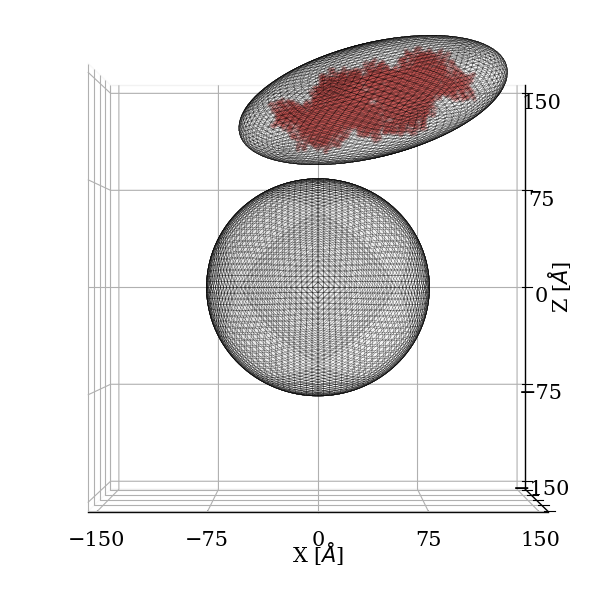
\includegraphics[width=0.65\textwidth]{viz/one_pca_full_display.png} 
    \caption{Sensor protein display: PCA ellipsoid with charges distribution located at $\pm 1$ nm of the 
    nanoparticle in the $z$-direction.}
    \label{fig:one_pca_sketch}
 \end{figure}


\begin{figure}%[h] %  figure placement: here, top, bottom, or page
    \centering
    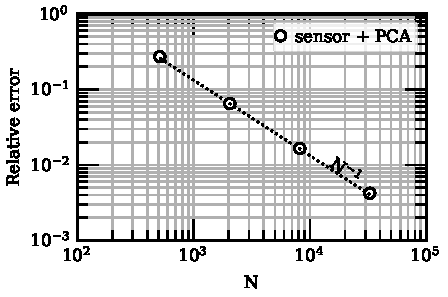
\includegraphics[width=0.85\textwidth]{convergence_sensor_pca_w380.pdf} 
    \caption{Grid-convergence study of extinction cross-section of a spherical silver
             nanoparticle with a PCA ellipsoid which contains 
             the charges distribution within it, located at $d=1$ nm.}
    \label{fig:err_sph-pca}
 \end{figure}

 \begin{table}%[h]
    \centering
    \caption{\label{table:err_sph-pca} Estimated percentage error of the PCA ellipsoid-sensor 
    system, with respect to the extrapolated value (using Richardson extrapolation).} 
    \begin{tabular}{c c}
    \hline%\toprule
    N & \% error \\
    \hline%\midrule
     $512$ & $27.2$ \\
     $2048$ & $6.5$ \\
     $8192$ & $1.66$ \\
     $32768$ & $0.42$ \\
    \hline%\bottomrule
    \end{tabular}
\end{table}

After performing the convergence analysis studies, we relaxed the numerical parameters of the computations to reduce the run-time without 
compromising accuracy. The following parameters were used to obtain all non-convergence results presented from now on for the case of PCA ellipsoids.

\begin{table}%[h]
    \centering
    \caption{\label{table:rel_pca_par} Relaxed parameters for the PCA ellipsoid case. The parameters that are not 
    mentioned here remain the same as in the convergence study.} 
    \begin{tabular}{c c}
    \hline%\toprule
    parameter & \% value \\
    \hline%\midrule
     $N_{sensor}$ & $8192$ \\
     $k_{fine}$ & $19$ \\
     $P$ & $6$ \\
     $tol$ & $1\times 10^{-3}$ \\
    \hline%\bottomrule
    \end{tabular}
\end{table}

The Richardson extrapolated value for the PCA case is: $1432.6561$ nm$^2$ and the computed value with the relaxed parameters 
is $1456.0781$ nm$^2$, giving us a percentage error of $1.63 \%$. 

\subsubsection{Charges model analysis} \label{ssub:pqr_analysis}

In order to know if we could use a volume equivalent (VE) approach we studied the effect of the charges inside the protein. We analyzed
the different representations of charges (full distribution and equivalent monopole), as well as the impact of having
no charges. The setup of the simulations consists of a silver sphere sensor ($r=8$ nm) with a PCA ellipsoid 
at $1$ nm of the surface of the sensor in the $z$-direction, oriented such that the dipole moment is aligned with the $y$-axis. We run 
three different cases, one with the full distribution of charges, a second case with one equivalent charge located in the
"center of mass" (See Figure \ref{fig:one_pca_cm_sketch}), and an ellipsoid with no charges. Figure 
\ref{fig:pqr_pca} shows the results for the different cases.

\begin{figure}%[h] %  figure placement: here, top, bottom, or page
    \centering
    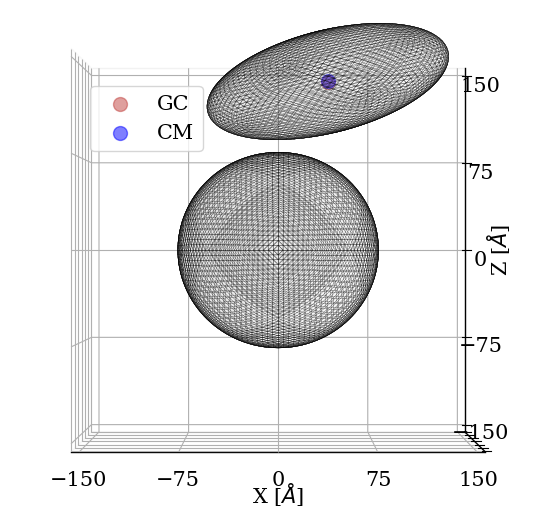
\includegraphics[width=0.65\textwidth]{viz/one_pca_cm_gc_display.png} 
    \caption{Sensor protein display: PCA ellipsoid with equivalent monopole charge, located at $\pm 1$ nm of the 
    nanoparticle in the $z$-direction. The label "CM" indicates the center of mass where the monopole charge is located, and
    the label "GC" indicates the geometric center for reference.}
    \label{fig:one_pca_cm_sketch}
 \end{figure}

 The resonance peak in all the curves in Figure \ref{fig:pqr_pca} occurs at $385.25$ nm. The 
 maximum value of the extinction cross section for the full distribution ("Full pqr") is $3827.06$ nm$^2$ and for 
 the monopole/center-of-mass representation ("CM pqr") is $3828.21$ nm$^2$, what results in a difference of $0.03 \,\%$. The
 maximum value of the extinction cross section when there are no charges present ("No pqr") is $3755.51$ nm$^2$ which compared to 
 the maximum for the full distribution gives us a difference of $1.87 \,\%$. Looking at these results we can say that the presence of 
 charges inside the protein does not affect the wavelength shift. However, it does affect the intensity of the maximum value of the 
 extinction cross section by approximately $2 \,\%$. Finally, we can say that using a monopole approximation for the distribution of charges, 
 is equivalent to using the full distribution of charges. Therefore, we will use the monopole charge model when doing computations with 
 a volume equivalent ellipsoid. 

\begin{figure}%[h] %  figure placement: here, top, bottom, or page
    \centering
    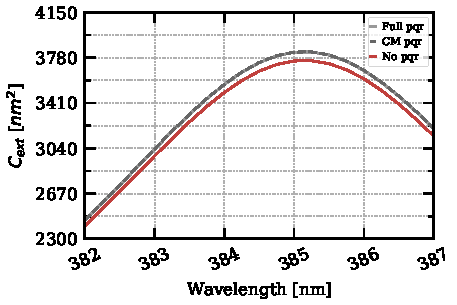
\includegraphics[width=0.85\textwidth]{pqr_analysis_pca.pdf} 
    \caption{Extinction cross-section as a function of wavelength for an $8$ nm
    silver sphere immersed in water with one PCA ellipsoid at $1$ nm away from 
    the surface in the $z$-direction, under a constant electric field on the $z$-direction.
    The label "Full pqr" corresponds to the full distribution of charges, the label "CM pqr" corresponds to a monopole representation 
    of the charges obtained by computing the center of mass of them, and the label "No pqr" 
    corresponds to the case where there are no charges present.}
    \label{fig:pqr_pca}
 \end{figure}



\subsection{Surface equivalent vs Volume equivalent model} \label{ssec:surf_vol_ell}

In section \ref{ssub:pqr_analysis} we show that using a monopole approximation is equivalent to using the full distribution of charges. This 
allows us to explore the effects of the volume equivalent model. Similarly to the PCA case, we present a convergence study for the volume  n section \ref{sssec:ve_conv}. 
Following the convergence study of the volume equivalent ellipsoid we show, in section \ref{sssec:ell_mod_comp}, the comparison of the PCA ellipsoid model and the volume equivalent 
model with the original BSA protein structure model, replicating the configuration shown in Figure \ref{fig:display_z}. 

\subsubsection{Volume Equivalent ellipsoid convergence analysis}\label{sssec:ve_conv}

We performed a grid convergence analysis on the VE (volume equivalent) ellipsoid - sensor system containing a monopole charge located 
in the center of mass of the charge distribution. (see Figure \ref{fig:one_ve_sketch}). Since we compute the extinction cross section of the sensor 
(8 nm radius silver sphere), we set a fixed mesh density for the ellipsoid and refine 
the mesh of the sphere ($N=512, 2048, 8192, 32768$). We found that a mesh with $N=1280$ elements for the ellipsoid was fine enough for the convergence study.
We used the same physical conditions and parameters that were used for the BSA-nanoparticle convergence analysis presented in
\ref{sec:grid_conv_bsa}. Similarly to the BSA-sensor system, the distance between the sensor and the VE-ellipsoid 
was $d=1$ nm, and the ellipsoid was oriented such that the dipole moment of the charges was aligned with the $y$-axis. To obtain the error 
estimate we used Richardson extrapolated value of the extinction cross section as a reference, $C_{ext} = 1683.8117$ nm$^2$. Table \ref{table:err_sph-ve} shows 
the percentages error for the different meshes used in this study. The observed order of convergence is $0.99$, and Figure \ref{fig:err_sph-ve} shows that the error decays 
with the number of boundary elements ($1/N$). This provides evidence that the numerical solutions computed with \pygbe are correctly resolved by the meshes.  

\begin{figure}%[h] %  figure placement: here, top, bottom, or page
    \centering
    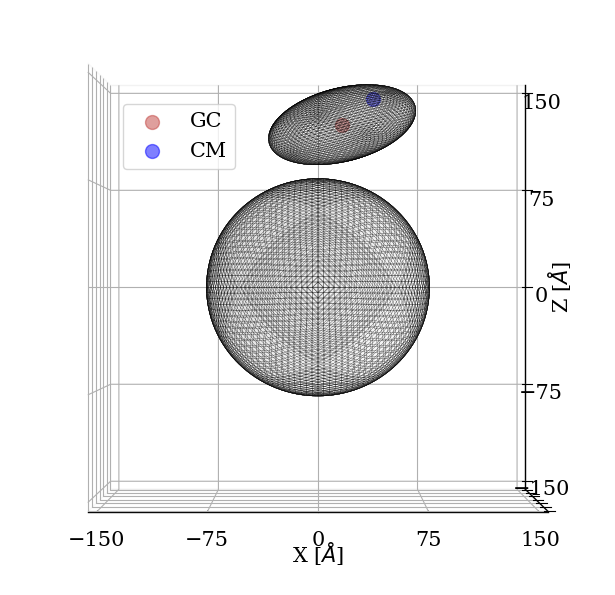
\includegraphics[width=0.65\textwidth]{viz/one_ve_cm_gc_display.png} 
    \caption{Sensor protein display: Volume equivalent ellipsoid with monopole charge ("CM"), located at $1$ nm of the 
    nanoparticle in the $z$-direction. The geometric center ("GC") is displayed for reference.}
    \label{fig:one_ve_sketch}
 \end{figure}


\begin{figure}%[h] %  figure placement: here, top, bottom, or page
    \centering
    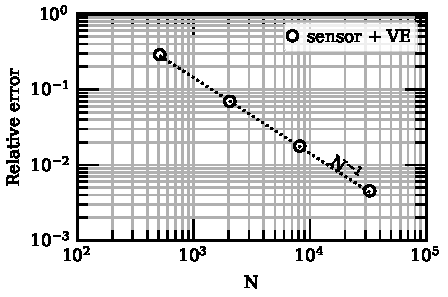
\includegraphics[width=0.85\textwidth]{convergence_sensor_ve_w380.pdf} 
    \caption{Grid-convergence study of extinction cross-section of a spherical silver
             nanoparticle with a volume equivalent ellipsoid at $d=1$ nm which contains 
             a monopole charge.}
    \label{fig:err_sph-ve}
 \end{figure}

 \begin{table}%[h]
    \centering
    \caption{\label{table:err_sph-ve} Estimated percentage error of the VE ellipsoid-sensor 
    system, with respect to the extrapolated value (using Richardson extrapolation).} 
    \begin{tabular}{c c}
    \hline%\toprule
    N & \% error \\
    \hline%\midrule
     $512$ & $28.8$ \\
     $2048$ & $6.96$ \\
     $8192$ & $1.78$ \\
     $32768$ & $0.45$ \\
    \hline%\bottomrule
    \end{tabular}
\end{table}

After performing the convergence analysis studies, we relaxed the numerical parameters of the computations to reduce the runtime without 
compromising accuracy. We use the parameters from Table \ref{table:rel_pca_par} to obtain all non-convergence results presented from 
now on for the case of VE ellipsoids. The Richardson extrapolated value for the VE case is: $1683.8117$ nm$^2$ and the computed value with 
the relaxed parameters is $1713.1972$ nm$^2$. If we compute the percentage error we obtain $1.75 \%$.

\subsubsection{Ellipsoid model vs original BSA}\label{sssec:ell_mod_comp}

In Figure \ref{fig:2pz_ell_resp} we show the results of comparing both ellipsoidal models of the protein with the 
original representation of the protein obtained from the crystal structure. We present the LSPR response 
of the system shown in Figure \ref{fig:display_z}, and for the ellipsoidal models we use an equivalent 
setup that replaces the proteins, located at $\pm 1$ nm in the $z$-direction, for the respective ellipsoids.
Both the PCA and VE model contain a monopole charge in the center of mass of the distribution. These results reveal 
the model chosen to represent the analytes matters.

\begin{figure} %[h] %  figure placement: here, top, bottom, or page
    \centering
    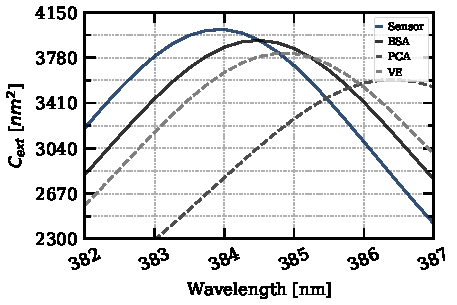
\includegraphics[width=0.85\textwidth]{two_ell_analysis.pdf} 
    \caption{Extinction cross-section as a function of wavelength for a 8 nm silver sphere immersed 
    in water with two BSA proteins ("BSA"), two PCA-ellipsoids with one equivalent charge ("PCA"), and two
    volume equivalent ellipsoids ("VE") with one equivalent charge. In all cases the proteins or equivalents
    are placed at $\pm 1$ nm away from the surface in the $z$-direction, except for the case where there is 
    no protein ("Sensor").}
    \label{fig:2pz_ell_resp}
 \end{figure}

The PCA model (surface based model, surface of PCA is $1.14$ times the original surface) over estimates the LSPR response, 
with a shift of $2.5$ nm ($400\%$ more) than the original shift ($0.5$ nm). The VE model (volume based based)  
overestimates the original by $50\%$ (shift $0.75$ nm), but we can say that a reduced order model based on the volume 
is a closer representation of the full protein. In both cases we see that the intensity of the peak decreases. This can be 
a problem, along with the overestimation of the shift, if the results are intended for use in the computation of sensitivity. The Figure of
Merit is usually how a nanoparticle's sensing capabilities are characterized, and is defined as the ratio between the 
sensitivity ($S = \Delta \lambda / \Delta n$) over the full width mid height (FWMH) \cite{otte2012}. Making 
conclusions of sensitive capabilities of sensors, based on models that underestimate the magnitude of the peak and 
overestimate the shift, can lead to incorrect assessments.

In summary, using an ellipsoidal shape of equivalent surface that contains all charges is not a good approximation
since it overestimates the shift considerably. The VE-equivalent model exhibits a shift of $0.75$ nm, which is still  
an overestimated response. However, we believe that the volume equivalent approximation can be used to investigate 
qualitative behaviors and take advantage of less expensive simulations to get insights on the physics of problems 
that might be impossible to simulate due to memory restrictions.

\subsection{Other model considerations}

Besides the effect of the surface and the volume based model as an approximation of the protein, there are other
factors that can affect the behavior of the system sensor-BSA. In this section we present the results of choosing a spherical 
geometry instead of an ellipsoidal model, the results of the protein orientation, the number of proteins in the vicinity of the nanoparticle, and 
the effect of the magnitude of the incident electric field. 

\subsubsection{Sphere vs Ellipsoid for protein modeling}

Spheres are one of the most common geometries used to represent the protein \cite{SantiagoCordobaETal2011, UngerETal2009}. In this 
section we compare a spherical volume-equivalent model with the ellipsoidal volume-equivalent model used in section
\ref{ssec:surf_vol_ell}. Figure \ref{fig:sph_vs_ell_ve} shows the different LSPR responses of a silver nanoparticle of $8$ nm of radius, 
for the different models. The peak for both the ellipsoid and the sphere of equivalent volume, happens at $384.75$ nm, and the 
maximum extinction cross section is nearly the same for both cases (difference $<$0.5$\%$). For the sphere simulation, 
the monopole charge was located at the geometric center. It is worth mentioning that locating the monopole charge in the
geometric center instead of the center of mass, has no impact on the LSPR response. We run simulations of a volume-equivalent ellipsoid 
with the charge on the geometric center and resulted in no variation of the resonance. The difference between the intensities at 
the peak is $<1\%$ (computations results in reproducibility materials, section \ref{sec:repro_ell}).

\begin{figure} %[h] %  figure placement: here, top, bottom, or page
    \centering
    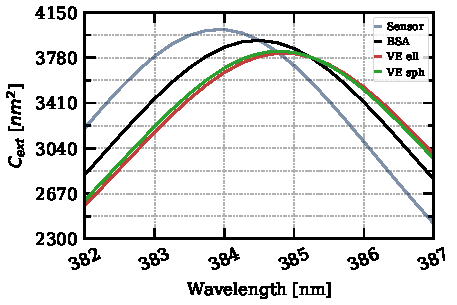
\includegraphics[width=0.85\textwidth]{two_ve_ell_sph_vs_BSA.pdf} 
    \caption{Extinction cross-section as a function of wavelength for an $8$ nm
    silver sphere immersed in water, under a constant electric field, with two volume equivalent 
    ellipsoids/spheres placed $\pm 1$ nm away from the surface in the $z$-direction.}
    \label{fig:sph_vs_ell_ve}
 \end{figure}

We still have the problem of overestimating the shift by $50$ $\%$ compared to the BSA protein original mesh, 
and at first sight we can consider this model comparable to the ellipsoidal volume-equivalent one. However, 
when we use a spherical model for the protein we lose any information regarding the orientation of the protein. 

\subsubsection{Effect of protein orientation}

Until this point we always kept the orientation of the proteins such that the dipole moment was parallel to the $y$-axis. In this 
section we explore the effects of protein orientation in respect to the nanoparticle in the LSPR response. For this study we use the 
volume equivalent ellipsoids in three different orientations: the original configuration where the dipole moment is parallel to 
the $y$-axis, a configuration such that the principal axis $a$ is parallel to $y$-axis, 
and finally a configuration where the principal axis $b$ is parallel to $y$ (see Figure \ref{fig:two_ve_conf_display} for configurations). 
 
 \begin{figure} %[h] %  figure placement: here, top, bottom, or page
    \centering
    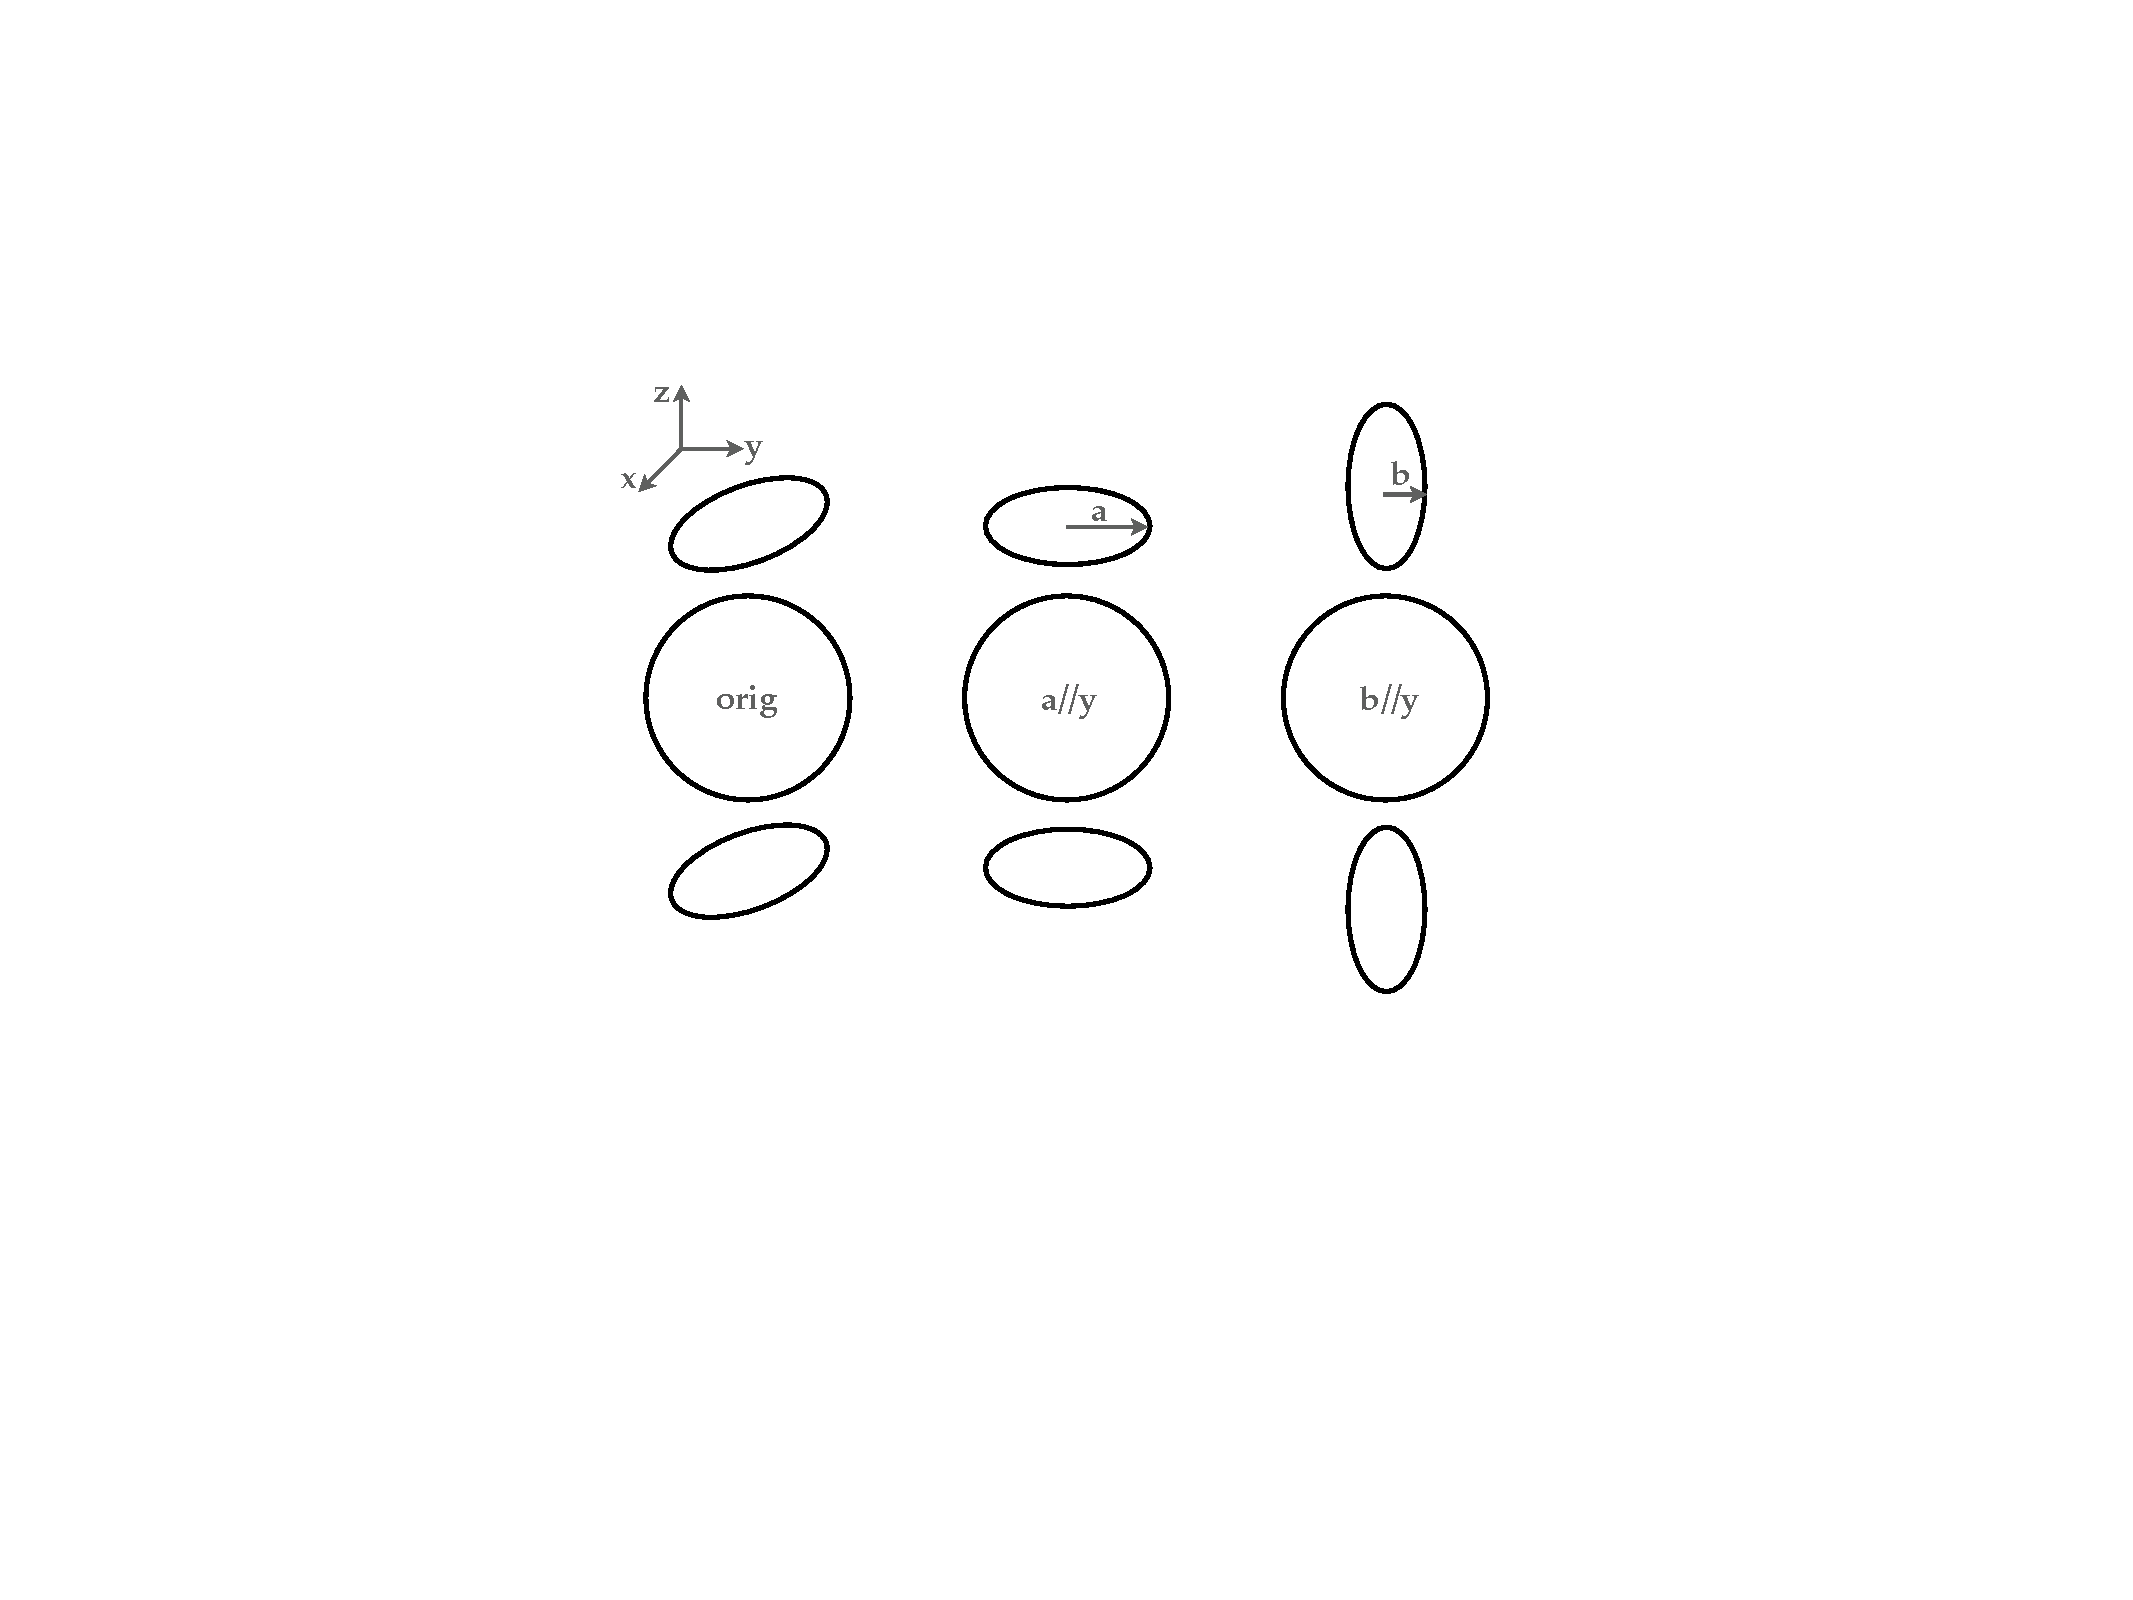
\includegraphics[width=0.65\textwidth]{viz/two_ve_conf_display.pdf} 
    \caption{Different configurations for two volume equivalent ellipsoids.}
    \label{fig:two_ve_conf_display}
 \end{figure}
 
 \begin{figure} %[h] %  figure placement: here, top, bottom, or page
     \centering
     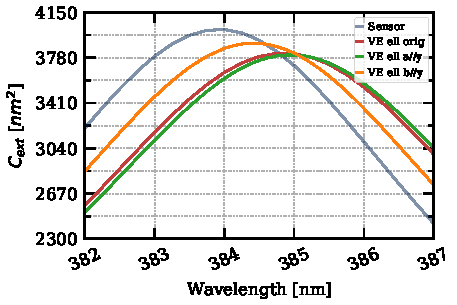
\includegraphics[width=0.85\textwidth]{two_ve_ell_mult_config.pdf} 
     \caption{Extinction cross-section as a function of wavelength for an $8$ nm
     silver sphere immersed in water, under a constant electric field, with two BSA ellipsoids placed 
     $\pm 1$ nm away from the surface in the $z$-direction. "VE ell orig": dipole moment parallel to the $y$-axis,
     "VE ell a//y": principal axis $a$ is parallel to $y$-axis, and "VE ell b//y": principal axis $b$ is parallel to $y$-axis}
     \label{fig:two_ell_mult_config}
  \end{figure}
 
Figure \ref{fig:two_ell_mult_config} shows the LSPR response of a silver nanoparticle when ellipsoids 
are placed in different positions and orientations. The peak when the dipole moment is parallel to the $y$-axis (original)
is $3815.72$ $nm^2$ and occurs at $384.75$ nm, causing a shift of $0.75$ nm. When the orientation of the ellipsoid 
is such that $a//y$, the maximum value is $3802.51$ $nm^2$ and it happens at $385$ nm, which results in a shift of 
$1$ nm. The final orientation we study is when $b//y$ which has a peak of $3898.10$ $nm^2$ at $384.375$ nm, resulting 
in a shift of $0.375$ nm. These results tell us that the orientation of the protein affects the LSPR response, we can 
see that the shifts vary depending on the orientation, as well as the intensity of the peak. When using a spherical model, 
all these effects are not captured due to the nature of the geometry, which can lead to misleading conclusions. Even though, 
we know that using a volume equivalent ellipsoid model overestimates the shift, it stills captures the effect of the orientation, making
it a better candidate compared to a simple sphere.

\subsubsection{Effect of number of proteins}

In this section we study the effect of having multiple proteins around the nanoparticle. Even though we know 
that volume equivalent ellipsoids overestimate the response, they still account for the effects of 
orientation and they can give us an estimation on how the LSPR response changes when having multiple 
ellipsoids. We use the same orientations shown in Figure \ref{fig:two_ve_conf_display} but we added ellipsoids 
at $\pm 1$ nm in the $x$ and $y$ directions too. Figure \ref{fig:mult_ell} shows the results of the LSPR response 
of six ellipsoids located at $\pm 1$ nm in the $x$, $y$, and $z$-axis, for the different configurations. 
 
\begin{figure} %[h] %  figure placement: here, top, bottom, or page
    \centering
    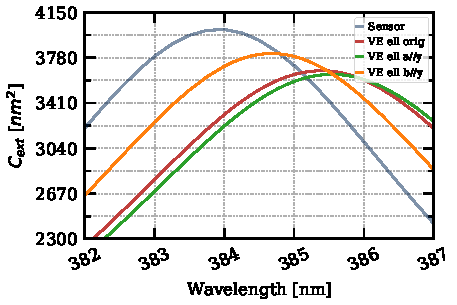
\includegraphics[width=0.85\textwidth]{six_ve_ell_mult_config.pdf} 
    \caption{Extinction cross-section as a function of wavelength for an $8$ nm
            silver sphere immersed in water, under a constant electric field, with multiple ellipsoids in different orientations 
            located at $\pm 1$ nm of the nanoparticle in the $x$, $y$ and $z$-axis.}
    \label{fig:mult_ell}
 \end{figure}

 The peak when the dipole moment is parallel to the $y$-axis (original) is $3673.89$ $nm^2$ and occurs at $385.375$ nm, causing a shift of 
 $1.375$ nm. When the orientation of the ellipsoid is such that $a//y$, the maximum value is $3643.97$ $nm^2$ and it
 happens at $385.5$ nm, which results in a shift of $1.5$ nm. The final orientation we study is when $b//y$ which 
 has a peak of $3814.23$ $nm^2$ at $384.625$ nm, resulting in a shift of $0.625$ nm. We can see that adding more proteins, 
 regardless of the orientation, increases the shift. However, depending on the orientation, the percentage of shift increment 
 varies. When we go from two ellipsoids on $\pm 1$ nm on the $z$-direction to six ellipsoids located at 
 $\pm 1$ nm in the $x$, $y$, and $z$-axis we see an increment on the shift of:
 
 \begin{itemize}
     \item {$~83\%$ when the dipole moment is parallel to the $y$-axis}
     \item {$50\%$ when the principal axis $a$ is parallel to the $y$-axis}
     \item {$~66.67\%$ when the principal axis $b$ is parallel to the $y$-axis}
 \end{itemize}    

These results tell us that the LSPR response is not only affected by the orientations but also by the number of proteins 
in the vicinity of the sensor. The addition of proteins, even though it always translates in a bigger shift, the increment  
is not linear, and it varies with the orientation. 

\subsubsection{Effect of magnitude of electric field}

Another factor that is involved in the computational model is the effect of the magnitude 
of the incident electric field. For all the simulations of this work we used the magnitude of the electric field from Phan and 
coworkers \cite{PhanETal2013}. In this section, we vary the magnitude of the electric field across several orders of magnitude 
and study its effect on the LSPR response. 

\begin{figure}%[t] %  figure placement: here, top, bottom, or page
    \centering
    \subfloat{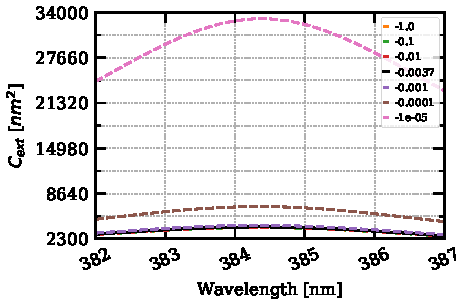
\includegraphics[width=0.85\textwidth]{VE_ell_cm_elec_field_var.pdf}}\\
    \subfloat{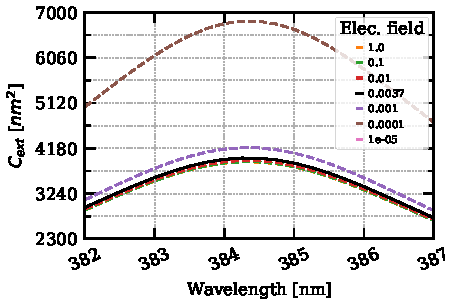
\includegraphics[width=0.85\textwidth]{VE_ell_cm_elec_field_var_zoom.pdf}} 
    \caption{Extinction cross-section as a function of wavelength for an $8$ nm
    silver sphere immersed in water, under a constant electric field, with a volume equivalent ellipsoid
    located at $1$ nm in the $z$-direction. The different colors represent different magnitudes of the 
    electric field where the units are $[e]/([{\text{\AA}}^2][\epsilon_0])$. The bottom figure is a zoom of the top 
    figure.}
    \label{fig:efield_effect}
 \end{figure}

Figure \ref{fig:efield_effect} shows how the magnitude of the incident electric field affects the LSPR response 
of a silver nanoparticle of radius $r=8$ nm when having a volume equivalent ellipsoid located 
$\pm 1$ nm in the $z$-direction (display Figure \ref{fig:one_ve_sketch}). We can see that as we decrease the magnitude of the electric field, 
the intensity of the extinction cross section increases. For all the different values of electric field except 
$1\times10^{-5}$ the peak occurs at $384.25$ nm, when the magnitude is $1\times10^{-5}$ the peak occurs at 
$384.5$ nm. This tells us that the magnitude of the electric field affects the shift. We computed 
the magnitude of the electric field due to the single charge inside the ellipsoid, on the surface of the nanoparticle,
and we found that its magnitude is $~5.4 \times 10^{-4}$ $[e]/([{\text{\AA}}^2][\epsilon_0])$. Therefore, 
when the magnitude of the incident electric field is smaller than the magnitude of the electric field generated by 
the protein on the surface of the nanoparticle, the shift increases. It is worth mentioning that if there are no charges 
present in the protein, the extinction cross section does not vary when the magnitude of the incident electric field 
changes. 


\section{Dielectric study}\label{sec:diel_study}

Most computational works in the literature use a constant real dielectric value both for the protein and the
embedding medium \cite{NghiemETal2012, SantiagoCordobaETal2011,UngerETal2009}. Such modeling does not account for the losses 
in that medium. LSPR biosensors detect a target molecule by monitoring plasmon resonance frequency changes due to the proximity 
of the target to the metallic nanoparticle. In this section, we show how the LSPR response changes when choosing different models 
for the dielectric in the protein and the medium around the system sensor-protein. We use the same setup used in chapter \ref{sec:lspr_response_bsa}
where we have two BSA proteins located at $\pm$ 1 nm on the $z$-direction of a silver nanoparticle of radius $r=8$ nm (see 
Figure \ref{fig:display_z}). The system sensor-protein is submerged in water and under a constant electric field of 
$0.0037$ $[e]/([{\text{\AA}}^2][\epsilon_0])$ in the $z$-direction. We first study the effect of having a real-valued dielectric 
for the protein, by keeping the water dielectric as complex. Second, we analyze the effect of the medium by using a real-valued 
dielectric, but we keep the BSA dielectric complex. Finally, we study the effect of certain combinations where both the medium 
and the protein have real-valued dielectrics. We obtained the values for the real dielectric of the BSA and water (medium) from the literature.
In most of the cases they provided the refractive index $n$, which we convert to the real dielectric $e_r=n^2$:  

\paragraph{BSA dielectric values:}
\begin{itemize}
    \item {Nghiem et al 2012 \cite{NghiemETal2012}: $n=1.9$, $e_r = n^2 = 3.61$}
    \item {Santiago-Cordoba et al 2011 \cite{SantiagoCordobaETal2011}: $n=1.45$, $e_r = n^2 = 2.0125$}
    \item {Phan et al 2013 \cite{PhanETal2013}: Average of real values of complex Lorentz-Drude model $e_r = 2.7498$}
\end{itemize}

\paragraph{Water dielectric values:}
\begin{itemize}
    \item {Real dielectric of water at room temperature $n=1.33$, $e_r = n^2 = 1.7689$}
    \item {Hale and Querry 1972 \cite{HaleQuerry1972}: Average of experimental real values $e_r = 1.7962$}
\end{itemize}
  
\subsection{BSA with real dielectric}

We study the effect of using a real-valued dielectric for the BSA, while keeping a complex-valued dielectric for the water where  
the system protein-sensor is embedded. Figure \ref{fig:bsa_diel} shows the extinction cross-section of silver nanoparticle 
of radius $r=8$ nm when having two BSA proteins located at $\pm1$ nm in the $z$-direction, for different dielectric models for the BSA. 
The computation of the original curve ("Complex") uses the complex dielectric for each frequency obtained from the Lorentz-Drude model 
from Phan et al. \cite{PhanETal2013}. The remaining curves correspond to the real-valued models from Santiago-Cordoba et al.\cite{SantiagoCordobaETal2011},
Nghiem et al \cite{NghiemETal2012}, and the average value of the real component from Phan et al. \cite{PhanETal2013}. The peak of the extinction cross section 
for both the complex model from Phan work \cite{PhanETal2013} and the average of its real part happen at $384.5$ nm, which represents a shift of $0.5$ nm from 
the LSRP response of the isolated nanoparticle. However, the intensity of the peak goes from $3901.06$ nm$^2$ to $4063.95$ nm$^2$ which is approximately a $~4.2\%$ increment. 
The resonance peaks for the values from Nghiem et al. and Santiago-Cordoba et al. occur at wavelengths $384.75$ nm and $384$ nm, respectively. These results 
translate in no shift for the case of Santiago-Cordoba et al., and a shift of $0.75$ nm for the case of Nghiem et al. The intensity for these two cases is 
bigger than the case where we used a complex dielectric for the model. 

\begin{figure} %[h] %  figure placement: here, top, bottom, or page
    \centering
    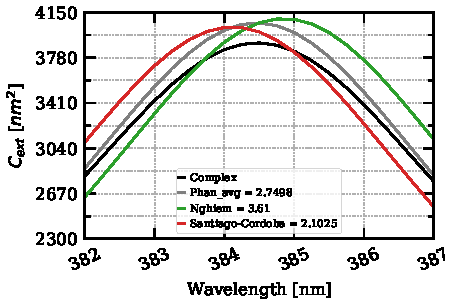
\includegraphics[width=0.85\textwidth]{bsa_diel_study.pdf} 
    \caption{Comparison of LSPR response of a silver nanoparticle to two BSA proteins located at $\pm1$ nm on the $z$-direction
    when using a complex vs a real dielectric for the protein.}
    \label{fig:bsa_diel}
 \end{figure}

The results from Figure \ref{fig:bsa_diel}, tell us that using a real dielectric for the protein affects the intensity of the extinction cross section. Using 
different values for the real dielectric also affects the LSPR response in terms of the shift. However, when comparing the complex model from Phan et al. versus
an average of the real parts of the dielectric, we see that the shift does not change. 

\subsection{Water with real dielectric}

After studying the effect of the dielectric model used inside the protein we explored the effects of the dielectric model in the 
embedding medium. We analyzed the effect of using a real-valued dielectric in the water when having the isolated nanoparticle (\ref{fig:iso_NP_diel}), 
as well as having the nanoparticle with two BSA proteins located at $\pm1$ nm on the $z$-direction (\ref{fig:real_w_comp_bsa}). We used
the complex dielectric values obtained from Hale and Querry \cite{HaleQuerry1972}, the average value of the real part from their work, and the real 
dielectric value for water at room temperature commonly used in the literature ("Generalization"). Figure \ref{fig:iso_NP_diel} shows
that using a complex representation of the dielectric versus using the average across the wavelengths of its real part, is indistinct. We can see that the curves
for the complex dielectric case (black curve) and the curve with average of the real part of the complex dielectric (green curve), match perfectly. However, when we
change the value of the real dielectric by a small amount (difference of $0.0273$), this has a big impact on where the peak occurs. For the "Generalization" case, where 
the dielectric is $1.7689$ we see that the peak occurs at a wavelength of $382.75$ nm, compared to the original peak for a dielectric of $1.7962$ which happens at $384$ nm. This shows
how sensitive is the LSPR response of the silver nanoparticle to the dielectric in which it is embedded. 
 
\begin{figure} %[h] %  figure placement: here, top, bottom, or page
    \centering
    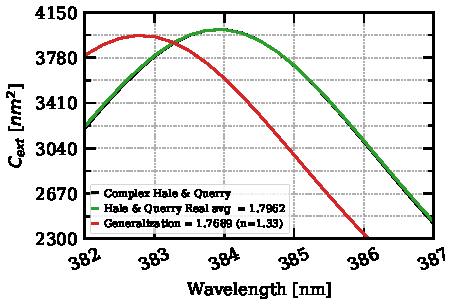
\includegraphics[width=0.85\textwidth]{iso_np_water_diel_study.pdf} 
    \caption{Comparison of LSPR response of isolated silver nanoparticle when using a complex 
     vs a real dielectric model for the water medium}
    \label{fig:iso_NP_diel}
 \end{figure}

Now that we understand how the dielectric model affects the LSPR response of the isolated nanoparticle, we can see how this 
effect varies when adding the BSA proteins at $\pm1$ nm on the $z$-direction. To isolate the effect of the dielectric model on the 
medium, we use the complex dielectric from Phan et al. \cite{PhanETal2013} for the BSA proteins. Figure \ref{fig:real_w_comp_bsa}
shows the shift in the LSPR response of a silver nanoparticle (dashed lines) when adding the BSA proteins (full lines), for the same 
real dielectrics models used in Figure \ref{fig:iso_NP_diel}. When using the average of the real part of the complex dielectric from 
Hale and Querry \cite{HaleQuerry1972} the shift is $0.5$ nm which is the same value compared to the full complex model. However, when using 
the generalization of the water dielectric (refractive index $n=1.33$), the peak for the extinction cross section when the two BSA proteins are
present occurs at a wavelength of $383.5$ nm, which gives us a shift in the LSPR response of $0.75$ nm. These results tell us that there is no 
difference in the LSPR response, wether we use the complex dielectric for the water or an averaged value of its real component. However, when using a
different real value for the dielectric, like the generalization $e=1.7689$, it not only affects the wavelength at which the resonance peaks occur
but also the shift when proteins are added in the vicinity. 

 \begin{figure} %[h] %  figure placement: here, top, bottom, or page
    \centering
    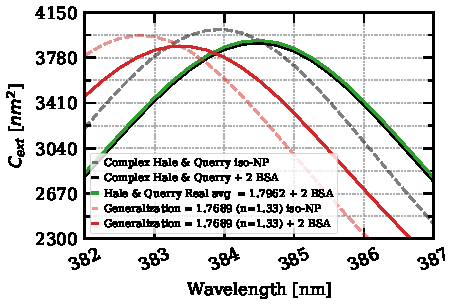
\includegraphics[width=0.85\textwidth]{bsa_w_real_water_diel.pdf} 
    \caption{Comparison of LSPR response of a silver nanoparticle to two BSA proteins located at $\pm1$ nm on the $z$-direction
    when using a complex vs real dielectric for the water medium.}
    \label{fig:real_w_comp_bsa}
 \end{figure}

 \subsection{BSA and water with real-valued dielectric}

Last but not least, we study the effect of using real-valued dielectrics for the BSA proteins as well as the water medium. For the BSA proteins 
we used the average value of the real component from Phan et al. \cite{PhanETal2013}, and for the water medium we used the same two dielectrics cases
used in the study of Figure \ref{fig:real_w_comp_bsa}. Figure \ref{fig:bsa_w_real} shows the results of using real dielectrics in both the proteins and
the water medium. The peaks in all cases occur at the same wavelengths compared to the case where we use a BSA complex dielectric for the protein, and as a 
consequence the shifts are the same than the ones reported in Figure \ref{fig:real_w_comp_bsa}. However, when we use real dielectric in both the medium 
and the proteins we see an increment in the magnitude of the extinction cross section of $~4.2\%$ for the Hale and Querry case, and $~3.6\%$ for the 
generalization case. These results tell us that, when it comes to the shift in the LSPR response, there is no difference between using a complex dielectric 
value for the protein and the medium, and using an averaged value of their real component. However, there is a difference in the magnitude of the 
extinction cross section that is a direct consequence of using a real-valued dielectric since this does not accounts for the losses in the medium. Similarly to the 
results shown in Figure \ref{fig:real_w_comp_bsa}, the usage of a different real dielectric for the water medium, changes where the peak occurs and the shift in the 
LSPR response. 

 \begin{figure} %[h] %  figure placement: here, top, bottom, or page
    \centering
    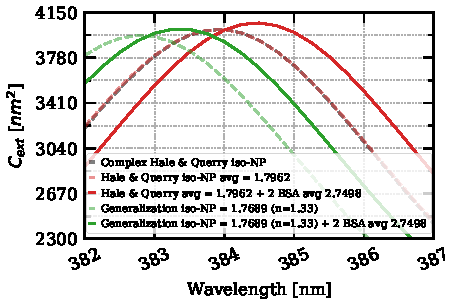
\includegraphics[width=0.85\textwidth]{bsa_phan_avg_real_water_diel.pdf} 
    \caption{Comparison of LSPR response of a silver nanoparticle to two BSA proteins located at $\pm1$ nm on the $z$-direction
    when using a real dielectric model in the protein and the water medium.}
    \label{fig:bsa_w_real}
 \end{figure}

In summary, when studying the LSPR response of a nanoparticle and how it shifts when proteins are in the vicinity, we can use 
real dielectrics for the water medium and the BSA protein, if they come from an average of the real part of the complex dielectric model 
or experimental data (see Hale and Quarry results on Figure \ref{fig:bsa_w_real}). However, when using real-valued dielectrics for the medium 
and the protein, the intensity of the extinction cross section increases, which is a problem if the results are intended to be used for 
sensitivity calculations. 

\section{Reproducibility and data management} \label{sec:repro_ell}
 
All the results of this chapter can be reproduced or replicated. \pygbe is openly developed and 
shared under the BSD3-clause license via its repository at \url{https://github.com/pygbe/pygbe}.

All results of this chapter were obtained on a lab workstation, built from parts. Hardware specifications are as follows:

\begin{itemize}
  \item CPU: Intel Core i7-5930K Haswell-E 6-Core 3.5GHz LGA 2011-v3
  \item RAM: G.SKILL Ripjaws 4 series 32GB (4 x 8GB)
  \item GPU: Nvidia Tesla K40c (with 12 GB memory)
\end{itemize}

Readers can reproduce all the figures in this chapter using the repro-packs shared in Zenodo. They include 
data and scripts needed to run the computations reported in this chapter, as well as Jupyter notebooks with 
all the plotting code:

{\color{red} PENDING}